The baseline for our evaluation is RocksDB -- a mature industry-leading KV-store implementation. 
\remove{RocksDB is used as storage layer of multiple popular SQL and NoSQL databases, e.g., MyRocks~\cite{MyRocks} (incarnation of MySQL) 
and MongoRocks~\cite{MongoRocks} (incarnation of MongoDB). RocksDB is an LSM-tree that is highly optimized for both read and write scenarios. 
For example, its compaction scheduling policies are highly tuned to minimize impact on mainstream data access.} 
We use the most recent RocksDB release 5.17.2, available Oct 24, 2018.  
It is worth noting that RocksDB's performance improved significantly during the last two years, primarily through 
optimized LSM compaction algorithms~\cite{CallaghanCompaction}.   We also compare against PebblesDB, 
a research LSM tree prototype that focuses on write amplification reduction and demonstrates advantage
over RocksDB in some scenarios~\cite{PebblesDB}. Finally, we experiment with TokuDB~\cite{TokuDB} -- 
the only publicly available KV-store whose design is based B$^\epsilon$-tree. However, TokuDB crashed 
in all executions with more then one thread, whereas in all single thread executions its performance was 
inferior to \sys's, hence these results are not presented.

The experiment setup is described in \cref{ssec:setup}. 
Performance results for \sys\ and RocksDB in 
different workloads are presented in \cref{ssec:results}. 
\cref{ssec:drill} analyzes \sys's sensitivity to different configuration settings and application parallelism. 
Finally, a comparison with PebblesDB is presented in \cref{ssec:pebbles}.
%\cref{ssec:recover} evaluates its recovery mechanism. 
 

\subsection{Setup}
\label{ssec:setup} 

\paragraph{Testbed.} We employ a C++ implementation~\cite{Cpp-YCSB} of YCSB~\cite{YCSB}, the  de facto standard  
benchmarking platform for KV-stores. 
YCSB provides a set of APIs and a workload suite. 
% Most modern KV-stores implement  YCSB adapter API's. 
%The platform decouples data access from workload generation, 
%thereby providing common ground for backend comparison. 

A YCSB workload is defined by  (1) the ratios of get, put, and scan accesses, 
and (2) a synthetic distribution of key access frequencies. 
YCSB  benchmarks  are inspired by real-life applications.
% and allows developing new ones through workload generation APIs. 
A typical YCSB experiment stress-tests the backend KV-store through a pool of concurrent worker threads that drive identical
workloads. %It aggregates the key performance metrics for the scenario under test.  

Our hardware is a 12-core Intel Xeon 5 machine with 4TB SSD disk. Unless otherwise stated, the YCSB driver  
exercises 12 workers. In order to guarantee a fair memory allocation to all KV-stores, 
we run each experiment within a Linux container with 16GB RAM. 

\paragraph{Metrics.} Our primary performance metrics are \emph{throughput} 
and \emph{latency percentiles}, as produced by YCSB. 
In addition, we measure \emph{write amplification}, namely, bytes written to storage over bytes passed from the application. 
%In order to explain the results, we also explore \emph{read amplification} (in terms of bytes as well as number of system calls per application read).  
%as well as the number of read \inred{ and write} system calls. 
%The OS performance counters are retrieved from the Linux proc filesystem. 

\paragraph{Workloads.} 
We vary the dataset size from 4GB to 64GB, in order to exercise multiple locality 
scenarios with respect to the available 16GB of RAM. Similarly to the published RocksDB benchmarks~\cite{RocksDBPerf}, 
we use a 10-byte decimal serialization of 32-bit keys, which that YCSB pads with a fixed 4-byte prefix (so effectively, 
the keys are 14 byte long), and 800-byte values. The data is stored uncompressed. 

We study the following key-access distributions:  

\begin{enumerate}
\item {\em Zipf-simple} -- the standard YCSB Zipfian distribution over simple (non-composite) keys. 
Key access frequencies are sampled from the heavy-tailed Zipf distribution, 
following the description in~\cite{Gray:1994:QGB:191839.191886}, with $\theta = 0.8$. 
The ranking is over a random permutation of the entire key range, so popular keys are uniformly dispersed.
% The key locations are sampled uniformly at random from the whole data range. 
This workload exhibits 
medium temporal locality (e.g., the most popular key's frequency is approximately $0.7\%$), 
and no spatial locality. 
%This is a standard YCSB workload that captures a multitude of use cases  -- e.g., a web page cache distribution by URL. 

\item {\em Zipf-composite}  -- a Zipfian distribution over composite keys. 
The key's $14$ most significant bits comprise the primary attribute. 
The primary attribute is drawn from a Zipf ($\theta=0.8$) distribution over its range, 
and  the remainder of the key is drawn uniformally at random.
Zipf-composite exhibits high spatial locality, representing workloads 
with composite keys, such as message threads~\cite{Borthakur:2011:AHG:1989323.1989438},
social network associations~\cite{Armstrong:2013:LDB:2463676.2465296}, and analytics databases~\cite{flurry}. 
\inred{(For completeness, we also experimented with other distributions of the key's suffix. 
The results were similar; only the primary dimension's distribution was significant for performance.)}

\item {\em Latest-simple} -- frequent access to recently added simple keys. 
Keys are inserted in sequential  order; the read keys' distribution is skewed towards recently added ones. 
Specifically, the sampled key's position wrt the most recent key is distributed Zipf. This is a 
standard YCSB workload with medium spatial and temporal locality which represents, e.g., status updates and reads. 

\inred{\item {\em Uniform} -- load of keys in random order (the keys are sampled uniformly at random). RocksDB
reports a similar benchmark~\cite{rocksdb-benchmarks}. }

\end{enumerate}

The workloads exercise different mixes of puts, gets, and scans. We use standard YCSB scenarios 
(A to F) that range from write-heavy ($50\%$ puts) to read-heavy ($95\%-100\%$ gets or scans). 
In order to stress the system even more on the write side, we introduce a new workload,  
YCSB-P, comprised of $100\%$ puts. It captures a non-sequential data load scenario (e.g., an ETL 
from an external data pipeline~\cite{flurry}). 

\paragraph{Evaluation methodology and configuration.} Each experiment consists of three stages. The first stage builds 
the dataset, by filling an initially empty store with a sequence of KV-pairs, ordered by key. The second phase is a warm-up phase running read-only operations to fill the caches. The third
phase exercises the specific scenario; all worker threads follow the same access pattern. Most experiments 
perform 80 million data accesses. The experiments that run scans perform 4 to 16 million accesses, depending 
on the scan size. We run 5 experiments for each data point, measure performance only during steady state (skipping load and warming phases), and present the median metric measurement %with confidence interval. 
\inred{(TODO: mention std. dev. - we won't show confidence intervals)}.

%\paragraph{Configuration.} 
We only present the performance metrics in asynchronous logging mode, since synchronous logging 
is approximately 10 times slower, thereby trivializing the results of every scenario that includes puts. 

All experiments in~\cref{ssec:results} use the same \sys\/ configuration, to avoid 
over-tuning; \cref{ssec:drill} provides insights on parameter choices.
We allocate 8GB to munks and 4GB to the row cache,
so together they consume 12GB out of the 16GB container. 
The row cache uses three hash tables.  
The Bloom filters for funks are partitioned 16-way.  
We set the \sys\/ chunk size limit to 10MB, and the rebalance threshold factor to $0.7$ -- i.e., 
chunks can grow up to 7MB  %(approximately 7000 KV-pairs) 
before being compacted. The funk log size limit is 2MB for munk-less chunks, 
and 20MB for chunks with munks. 

% \inred{for write intensive workloads, and 512KB for other workloads.}
We use RocksDB with the default configuration, which is also used by its public performance benchmarks~\cite{RocksDBPerf}.
\inred{Maybe mention we've evaluated various RocksDB mem configs?}

\subsection{\sys\ versus \ RocksDB}
\label{ssec:results} 

\begin{figure*}[tb]
\centering
\begin{subfigure}{0.33\linewidth}
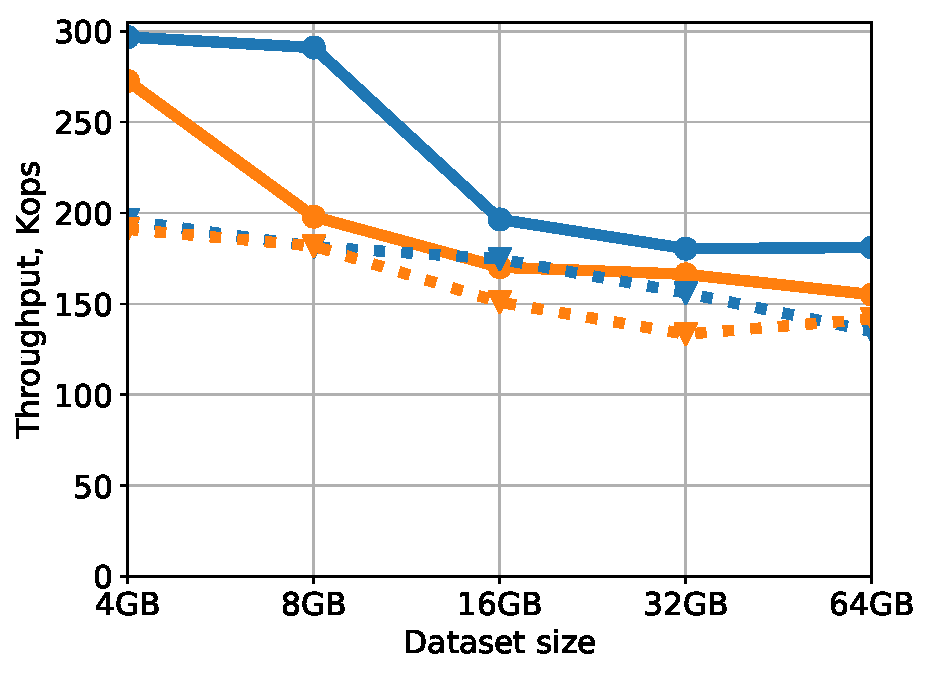
\includegraphics[width=\textwidth]{figs/Workload_P_line.pdf}
\caption{YCSB-P -- put-only}
\label{fig:throughput:p}
\end{subfigure}
\begin{subfigure}{0.33\linewidth}
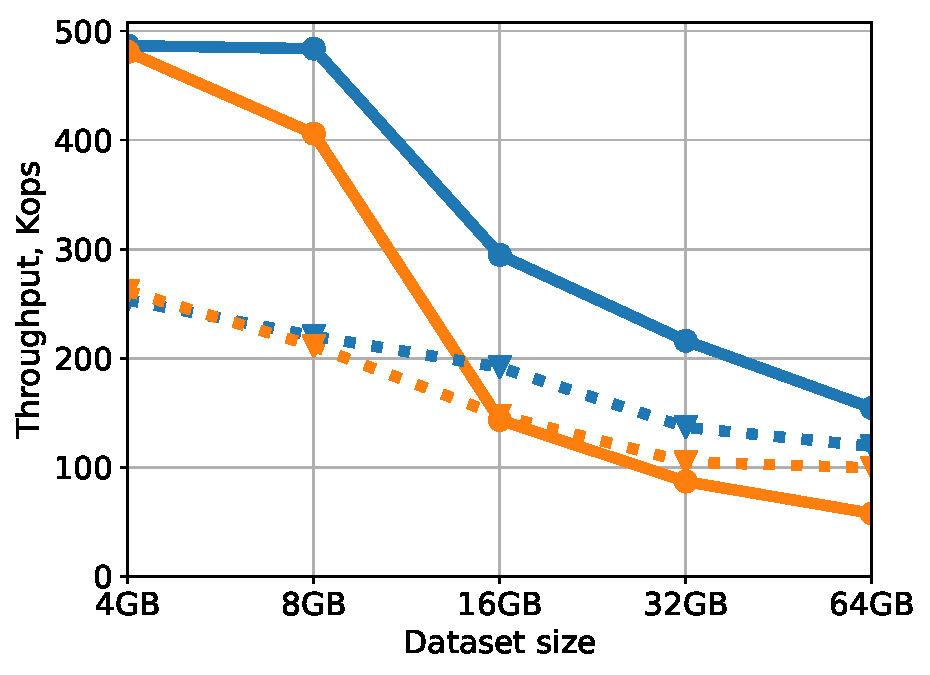
\includegraphics[width=\textwidth]{figs/Workload_A_line.pdf}
\caption{YCSB-A -- mixed get-put}
\label{fig:throughput:a}
\end{subfigure}
\begin{subfigure}{0.33\linewidth}
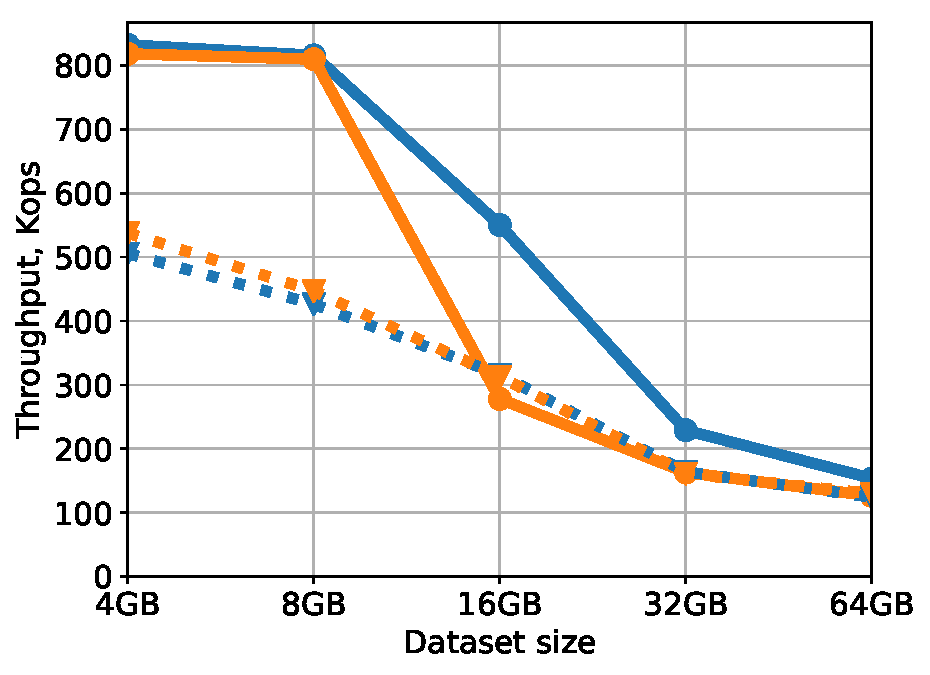
\includegraphics[width=\textwidth]{figs/Workload_B_line.pdf}
\caption{YCSB-B}
\label{fig:throughput:b}
\end{subfigure}
\hspace{70pt}
\begin{subfigure}{0.33\linewidth}
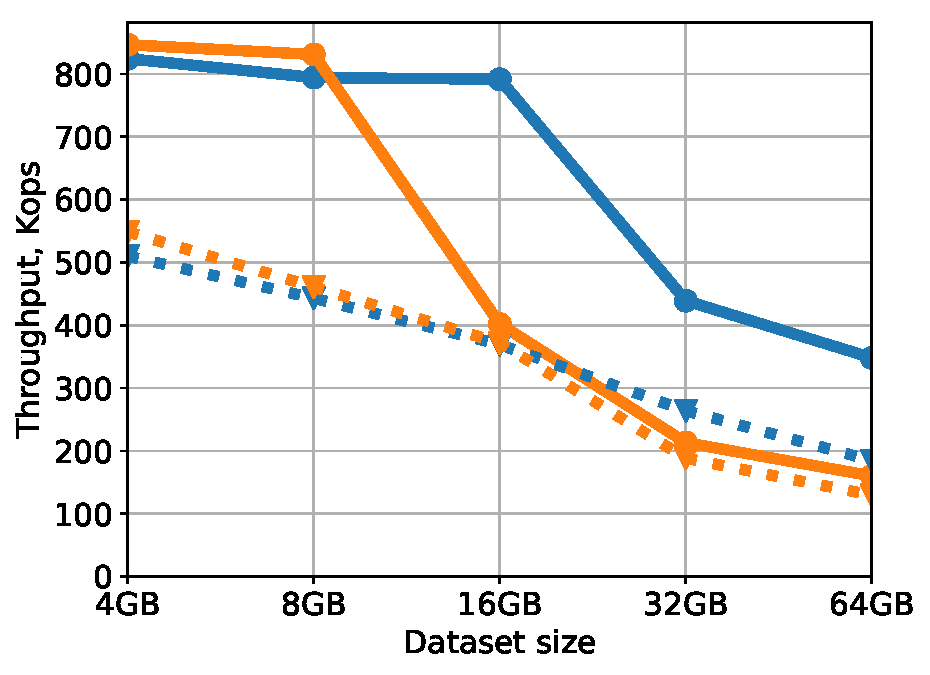
\includegraphics[width=\textwidth]{figs/Workload_C_line.pdf}
\caption{YCSB-C -- get-only}
\label{fig:throughput:c}
\end{subfigure}
\begin{subfigure}{0.33\linewidth}
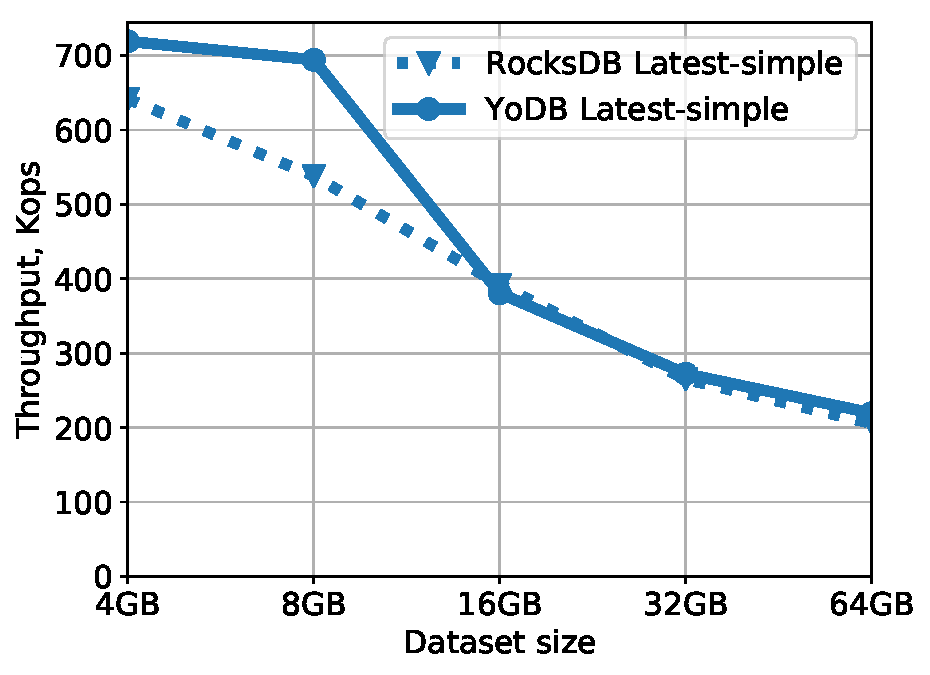
\includegraphics[width=\textwidth]{figs/Workload_D_line.pdf}
\caption{YCSB-D}
\label{fig:throughput:d}
\end{subfigure}
\begin{subfigure}{0.33\linewidth}
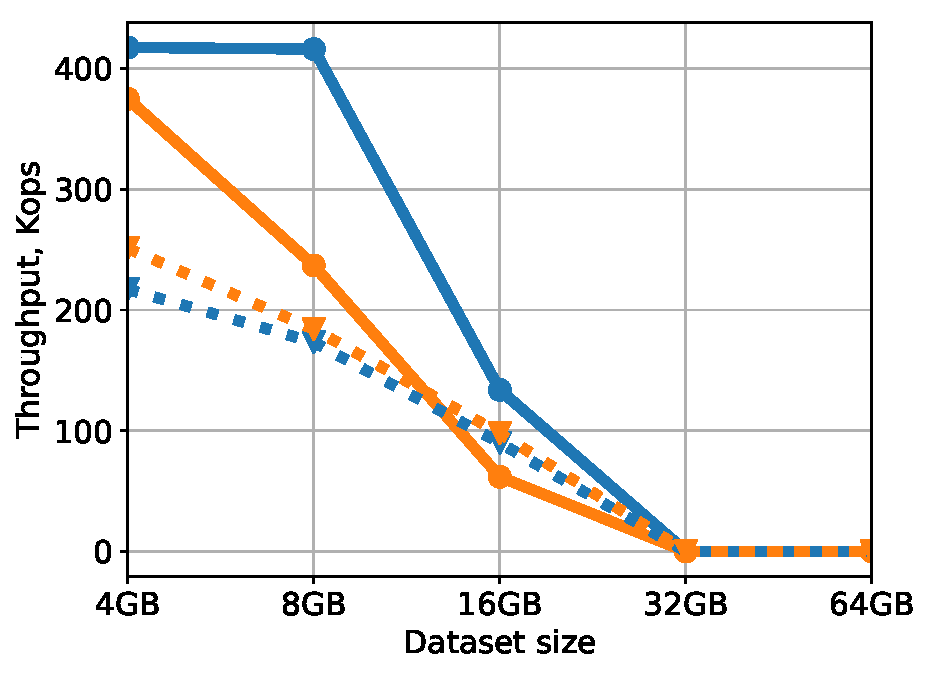
\includegraphics[width=\textwidth]{figs/Workload_F_line.pdf}
\caption{YCSB-F}
\label{fig:throughput:f}
\end{subfigure}
\hspace{70pt}
\begin{subfigure}{0.33\linewidth}
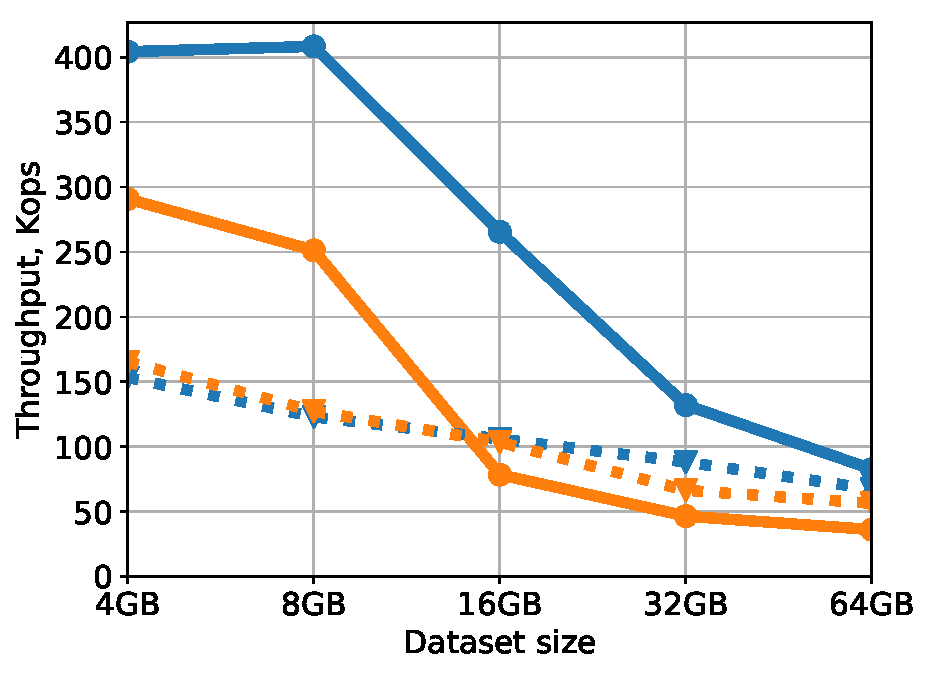
\includegraphics[width=\textwidth]{figs/Workload_E-_line.pdf}
\caption{YCSB-E10 -- short scans}
\label{fig:throughput:e10}
\end{subfigure}
\begin{subfigure}{0.33\linewidth}
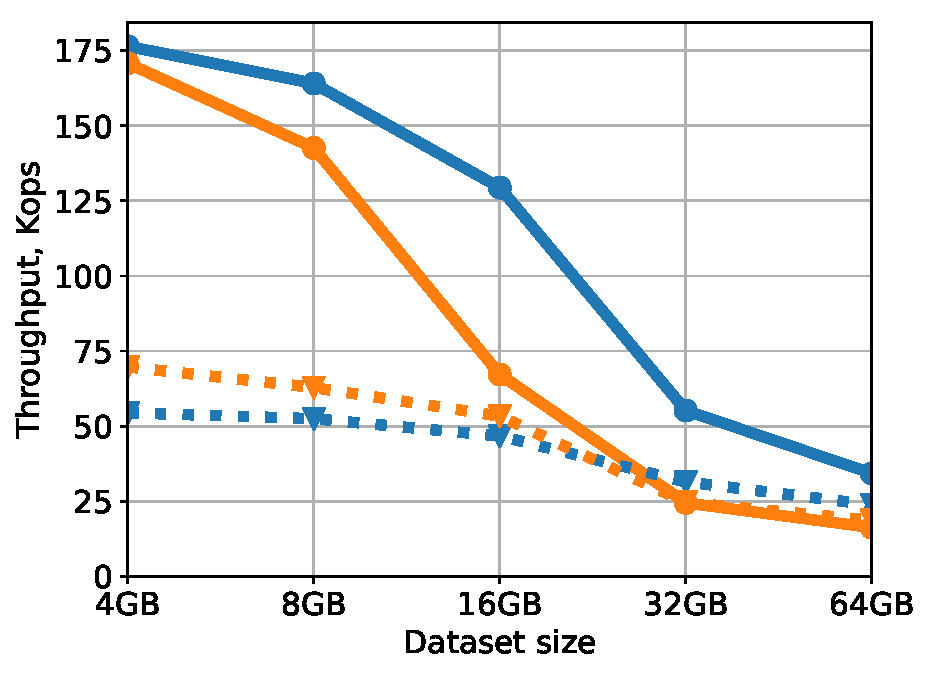
\includegraphics[width=\textwidth]{figs/Workload_E_line.pdf}
\caption{YCSB-E100 -- medium scans}
\label{fig:throughput:e100}
\end{subfigure}
\begin{subfigure}{0.33\linewidth}
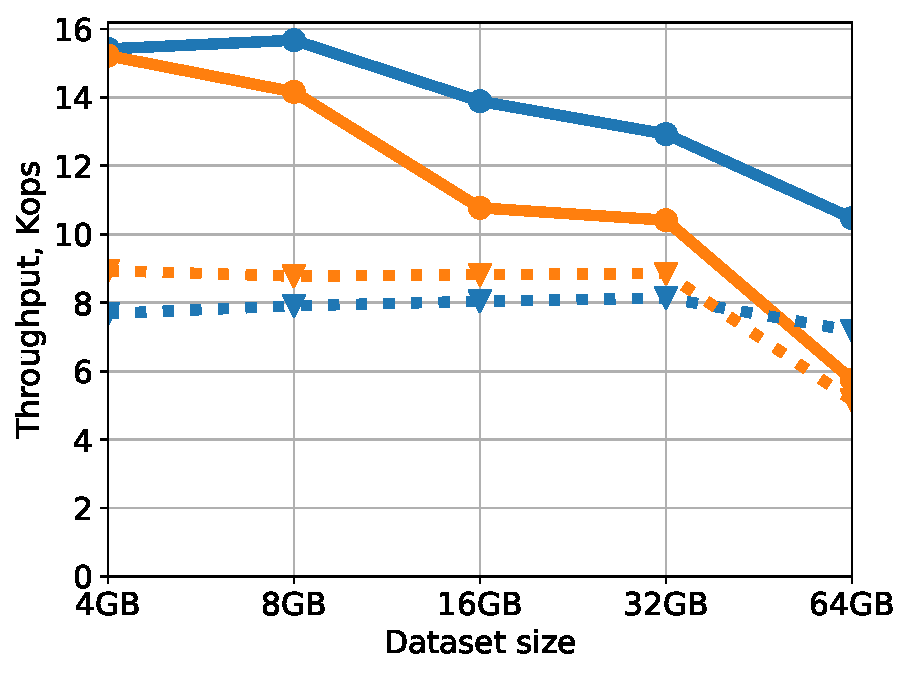
\includegraphics[width=\textwidth]{figs/Workload_E+_line.pdf}
\caption{YCSB-E1000 -- long scans}
\label{fig:throughput:e1000}
\end{subfigure}
\begin{subfigure}{\linewidth}
\centerline{

\includegraphics[width=0.9\textwidth]{figs/legend.pdf}
\vspace{-5mm}
}
\end{subfigure}
\caption{
{\sys\/ versus RocksDB throughput (Kops), under multiple workloads with Zipf distributions over composite (two-component) and
simple (non-composite) keys and scaling dataset sizes.}
}
\label{fig:throughput}
\end{figure*}

Figure~\ref{fig:throughput} presents throughput measurements under the Zipf-simple and 
Zipf-composite key distributions in the put-only workload YCSB-P, the mixed YCSB-A and YCSB-B, 
the get-only YCSB-C, the scan-heavy YCSB-E with three different scan sizes
and the read-modify-write workload YCSB-F.
%YCSB-B is omitted because the results are very close to those for YCSB-C. 
For completeness, we also experiment with YCSB-D that exercises the 
Latest workload -- frequent reads of the recently added simple keys. 
%The results are also close to YCSB-B, and omitted as well.

We now discuss the results for the different scenarios.

%YCSB-D exercises the Latest-simple  access pattern and its throughput is presented in Figure~\ref{fig:throughput:d}. 
  
{\bf Put-only.} 
In {YCSB-P} (100\% put, Figure~\ref{fig:throughput:p}), 
\sys's throughput is 1.3x to 2.3x versus RocksDB's with composite keys, 
and 0.7x to 1.6x with simple keys. 
\sys\ benefits from spatial locality whereas RocksDB's write performance 
is relatively insensitive to it, as is typical for LSM stores.

This workload's bottleneck is the reorganization of persistent data  
(funk rebalances in \sys, compactions in RocksDB), which causes 
write amplification and hampers performance. 
%The overhead manifests in disk write rates, which \sys\/ reduces through better use of spatial locality. 
For small datasets (8GB or less), \sys\/ accommodates all puts in munks, and so
funk rebalances are rare. In big datasets, funk rebalances do occur, but mostly in munk-less 
chunks, which are accessed less frequently than popular ones. 
Hence, in both cases, funk rebalances incur less I/O than RocksDB's compactions, which do not 
distinguish between hot and cold data. 

\sys\/'s high log size limit for chunks with munks 
also reduces I/O by decelerating munk flushes. This does not impact recovery time since \sys\/ 
does not replay its logs.

The write amplification in this workload is summarized in 
Table~\ref{fig:writeamp}. We see that \sys\/ reduces the disk write rate dramatically, 
with the largest gain observed for big datasets (e.g., $1.34$ versus $3.1$ for the 64GB 
database under Zipf-composite). Thus, \sys\/ also reduces disk wear.  


\begin{table}[htb]
\centerline{
{\small{
\begin{tabular}{lccccc}
\hline 
 & 4GB & 8GB & 16GB & 32GB & 64GB \\
\hline 
Zipf-composite: &  \multicolumn{5}{c}{}  \\
RocksDB & 2.08	& 2.29 & 2.35 & 2.40	& {\bf {3.10}}\\
\sys &  1.33	 & 1.30	& 1.22	& 1.25	& { {\bf 1.34}}\\
\hline 
Zipf-simple: &  \multicolumn{5}{c}{}   \\
RocksDB & 1.92	& 1.95 & 2.02 & 2.20	& 2.44 \\
\sys &  1.31	 & 1.27	& 1.08	& 1.20	& 1.19 \\
\hline 
\end{tabular}
}}
}
%\centering
%\hspace{0.05\linewidth}
%\begin{subfigure}{0.3\linewidth}
%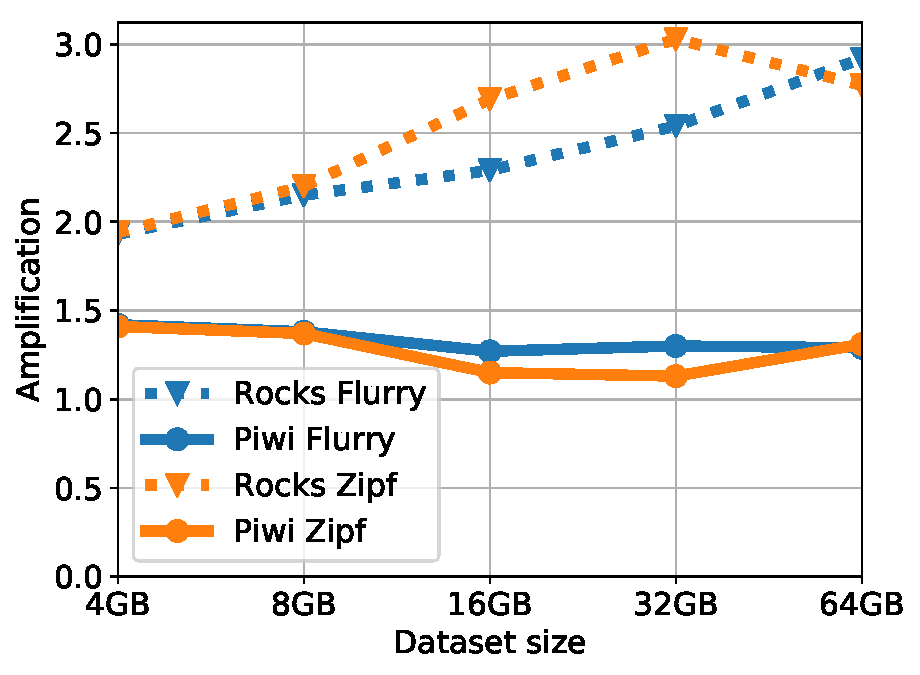
\includegraphics[width=0.3\textwidth]{figs/P_write_amplification_disk_line.pdf}
%\caption{YCSB-P}
%\label{fig:writeamp:p}
%\end{subfigure}
%\hspace{0.05\linewidth}
%\begin{subfigure}{0.3\linewidth}
%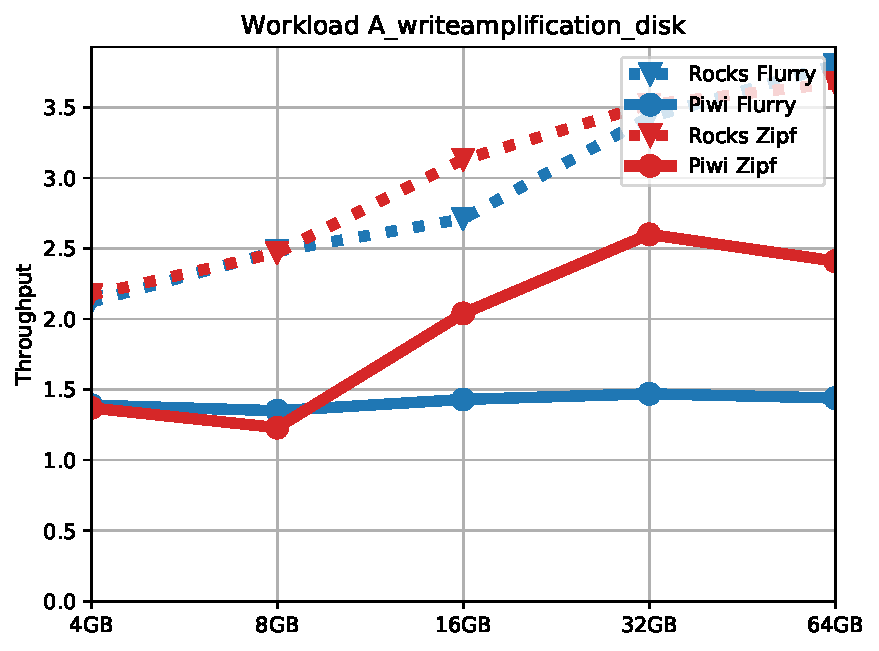
\includegraphics[width=\textwidth]{figs/Workload_A_writeamplification_disk_line.pdf}
%\caption{YCSB-A}
%\label{fig:writeamp:a}
%\end{subfigure}
\caption{{\sys\/ versus RocksDB write amplification under the put-only workload (YCSB-P) and scaling dataset sizes.}}
\label{fig:writeamp}
\end{table}

\inred{
	\sys\/ advantages are also evident when puts are uniformly distributed (green lines in Figure~\ref{fig:throughput:p}). Since funk rebalances are local, the distribution of rebalances (dictated by the distribution of puts) has little effect. In RocksDB, however, each L0 SST contains keys covering a wide range of keys, causing L0 to L1 compactions to include a large number of SSTs.
}

{\bf Mixed put-get.} YCSB-A (50\% put, 50\% get, Figure~\ref{fig:throughput:a})
 is particularly challenging for \sys\/ because it exercises a high contention between gets and puts. 
Here, the bottleneck is  disk search in gets, primarily the linear search in funk logs 
that keep filling up due to concurrent puts. (In-memory searches are three orders of magnitude faster.)

\sys\/ achieves $1.4$x to $3.2$x throughput versus RocksDB with composite keys, 
thanks to better exploitation of spatial locality. Figure~\ref{fig:tail_latency:co} shows that \sys\/
is also faster wrt the tail (95\%) put and get latency in this scenario. With simple keys,
\sys\/ is faster than RocksDB  for small datasets that fit in memory, and slower for big datasets.  
Figure~\ref{fig:tail_latency:si} zooms in on this setting: while \sys\/ is on par with 
RocksDB wrt the put latency in this setting, it falls short wrt the get latency.

When the working set does not fit in RAM, disk access dominates the tail latencies.
Figure~\ref{fig:readstat:dist} depicts the distribution of gets by the storage  component 
that fulfills the request, and Figure~\ref{fig:readstat:lat} presents the disk search latencies by component. 
For example, for the 64GB dataset, $3.3\%$ of gets are served from logs under Zipf-composite, versus $4.0\%$ under Zipf-simple,
and the respective log search latencies are $2.6$ ms vs $4.2$ ms. This happens because in the latter, puts are more dispersed, 
hence the funks are (1) cached less effectively by the OS, and (2) rebalanced less frequently so their logs grow longer.

\remove{
\begin{figure*}[tb]
\centering
\begin{subfigure}{0.36\linewidth}
\vskip .15in
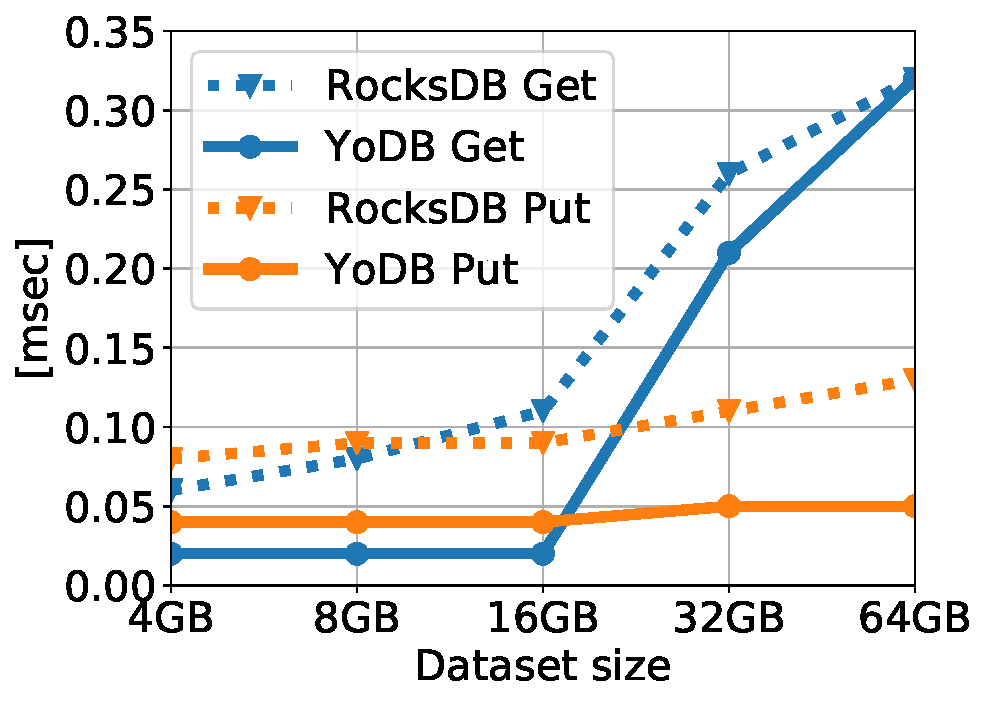
\includegraphics[width=\textwidth]{figs/tail_line.pdf}
\vskip .55in
\caption{95-percentile latency, put and get}
\label{fig:tail_latency:lat}
\end{subfigure}
\begin{subfigure}{0.32\linewidth}
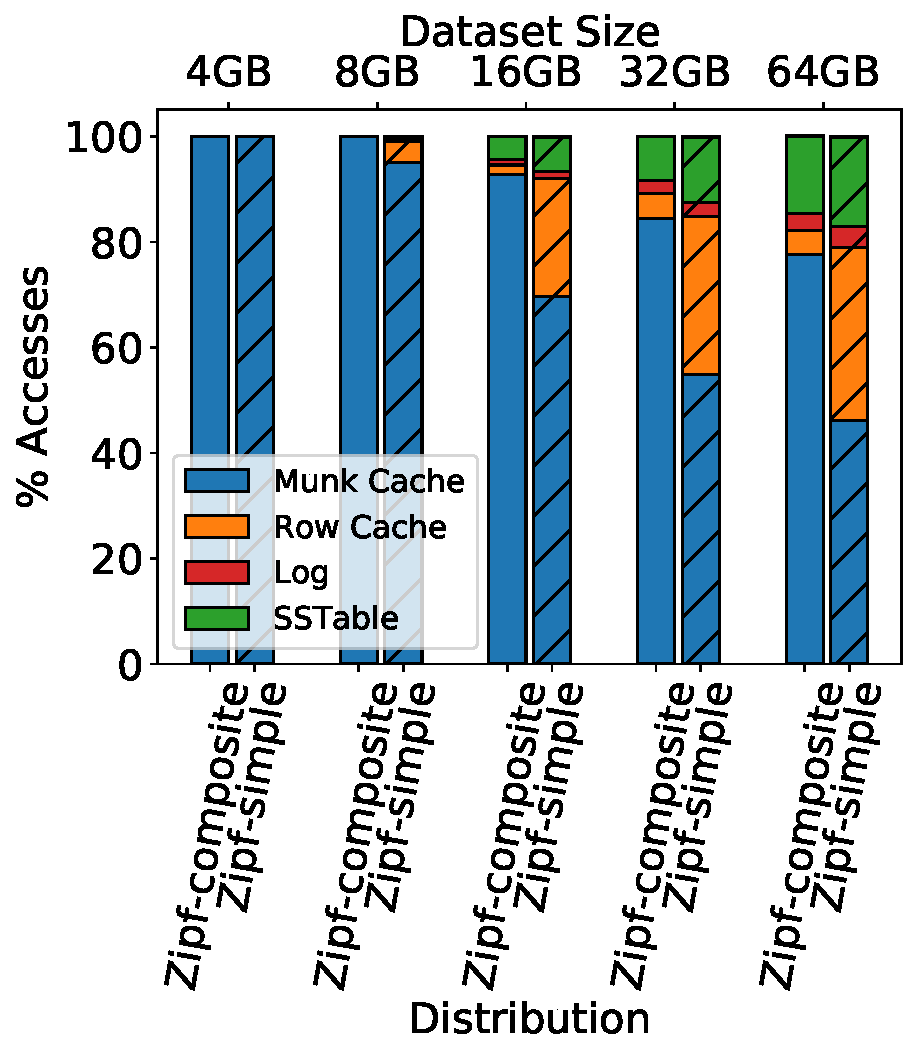
\includegraphics[width=\textwidth]{figs/Time_percentage_A.pdf}
\caption{Fraction of get accesses, by component}
\label{fig:tail_latency:dist}
\end{subfigure}
\begin{subfigure}{0.31\linewidth}
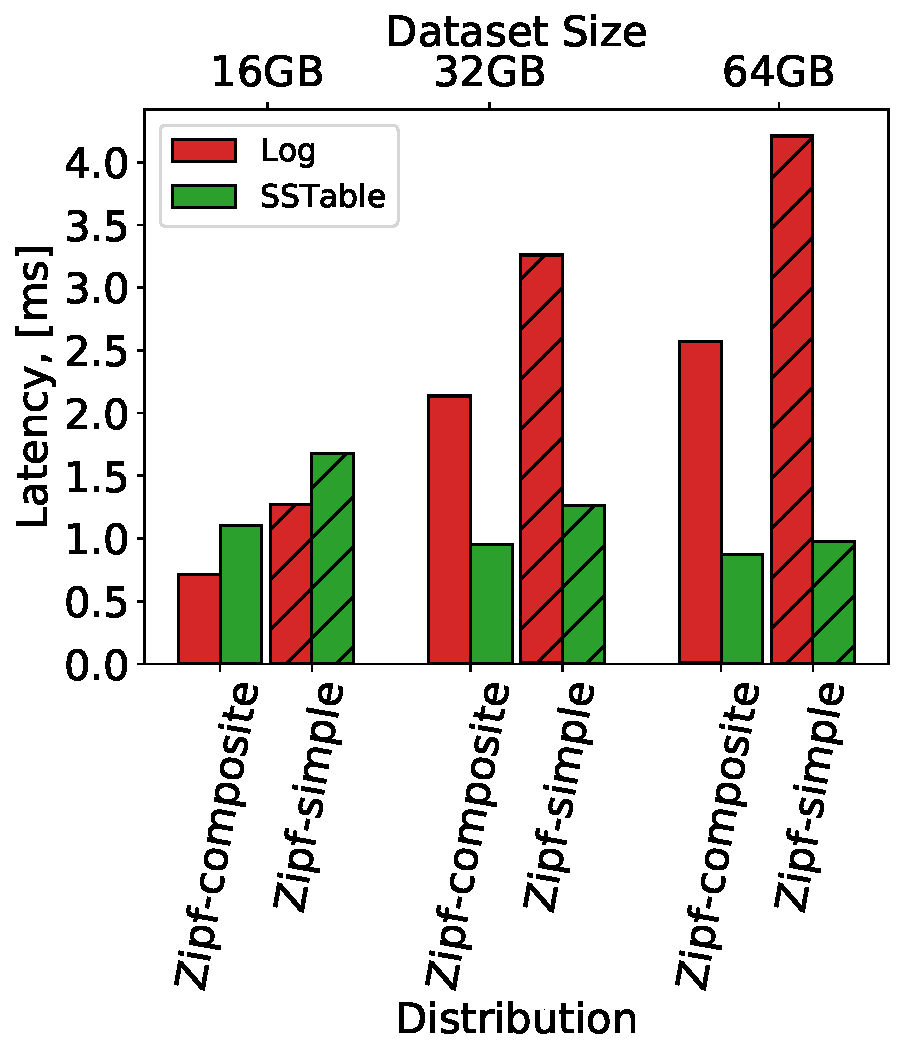
\includegraphics[width=\textwidth]{figs/Latency_A.pdf}
\caption{On-disk get latency, by component}
\label{fig:tail_latency:disk}
\end{subfigure}
\label{fig:tail_latency}
\caption{{\sys\/ tail latency analysis, under a mixed get-put workload (YCSB-A).}}
\end{figure*}
}

\begin{figure}[htb]
\centering
\begin{subfigure}{0.49\linewidth}
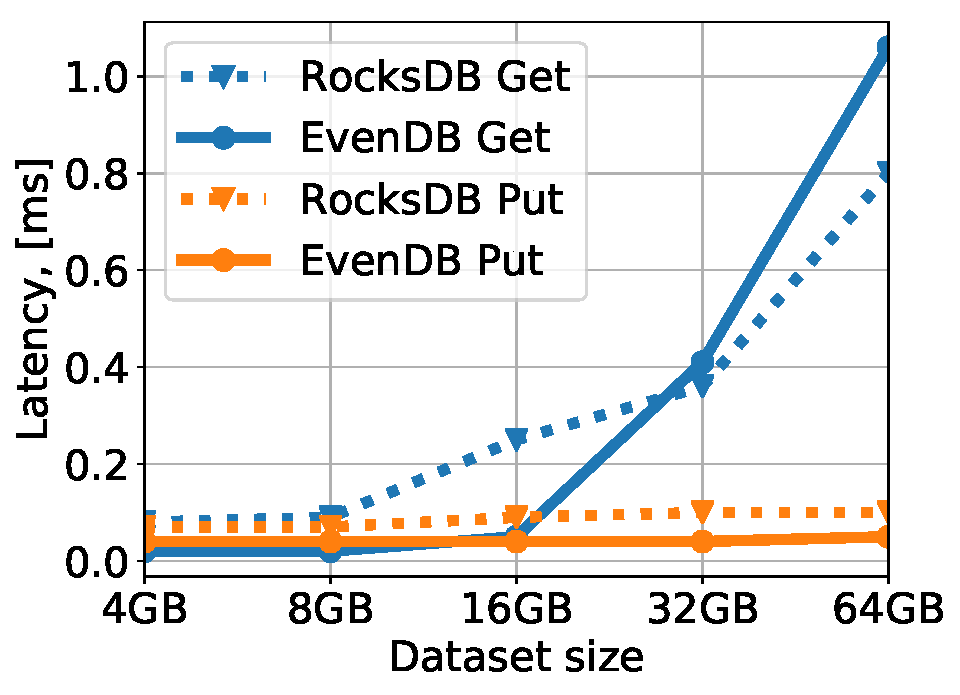
\includegraphics[width=\textwidth]{figs/tail_flurry_line.pdf}
\caption{Zipf-composite}
\label{fig:tail_latency:co}
\end{subfigure}
\begin{subfigure}{0.49\linewidth}
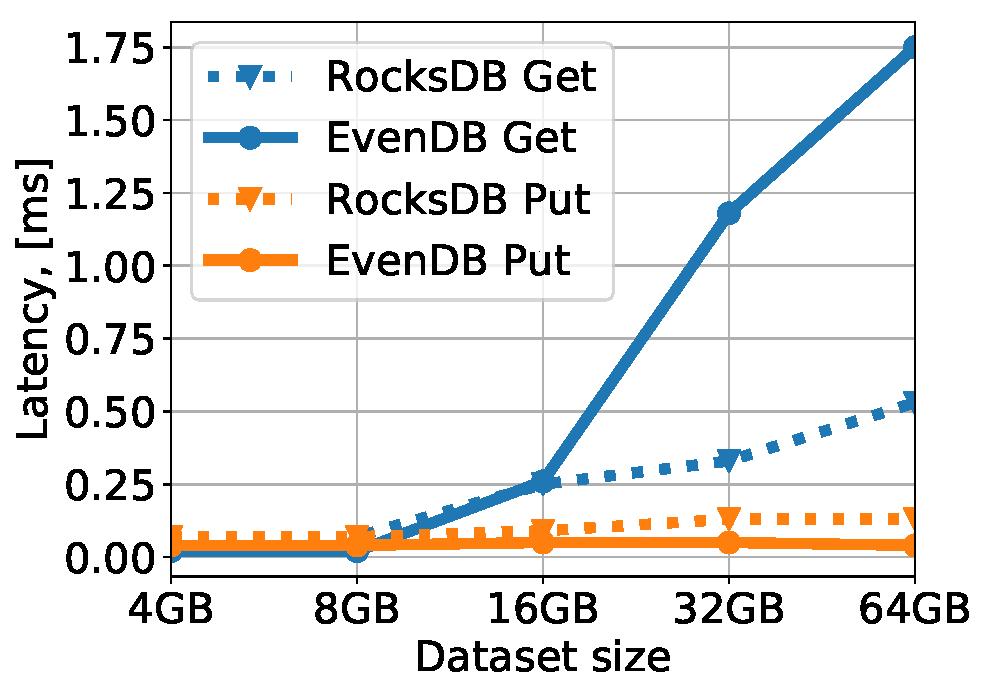
\includegraphics[width=\textwidth]{figs/tail_zipf_line.pdf}
\caption{Zipf-simple}
\label{fig:tail_latency:si}
\end{subfigure}
\caption{{\sys\/ versus RocksDB 95\% latency (ms), under a mixed get-put workload (YCSB-A).}}
\label{fig:tail_latency}
\end{figure}

\begin{figure}[htb]
\centering
%\hspace{0.05\linewidth}
\begin{subfigure}{0.5\linewidth}
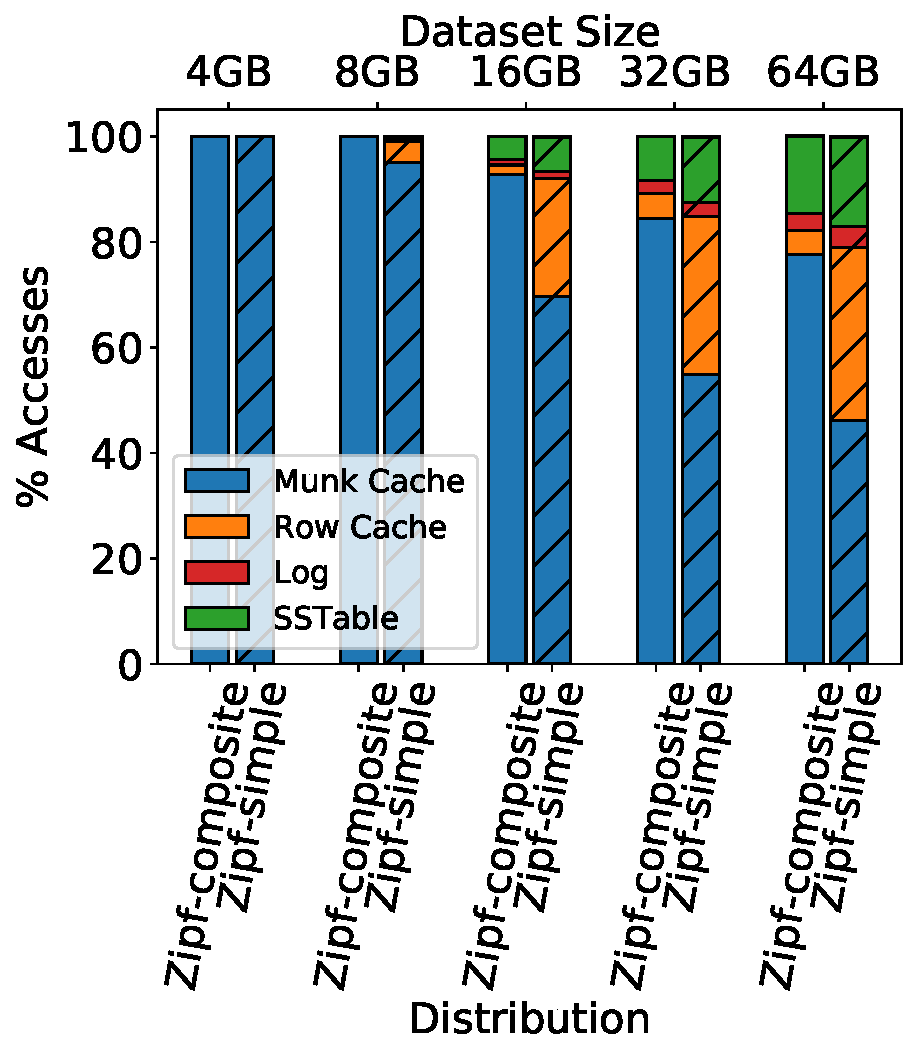
\includegraphics[width=\textwidth]{figs/Time_percentage_A.pdf}
\vskip .1in
\caption{Fraction of get accesses}
\label{fig:readstat:dist}
\end{subfigure}
%\hspace{0.05\linewidth}
\begin{subfigure}{0.49\linewidth}
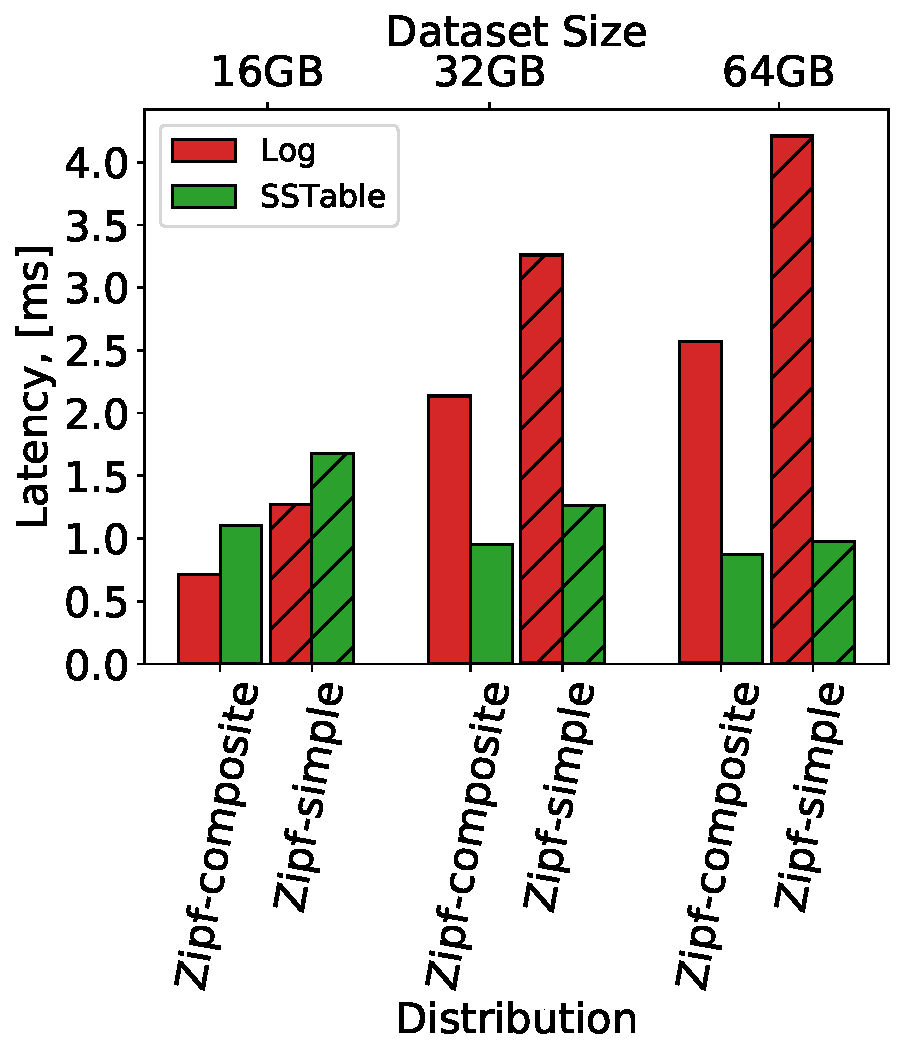
\includegraphics[width=\textwidth]{figs/Latency_A.pdf}
\caption{On-disk get access latency}
\label{fig:readstat:lat}
\end{subfigure}
\caption{{\sys\/ 95\% tail latency analysis by the serving component, under a mixed get-put workload (YCSB-A).}}
\label{fig:readstat}
\end{figure}

Naturally, the efficiency of in-memory caching is paramount. In the same example, the RAM hit rate 
(munk and row cache combined) is 
$82.1\%$ with composite keys versus $79\%$ without them. The row cache becomes instrumental as spatial locality drops --
 it serves $32.8\%$ of gets for Zipf-simple versus $4.5\%$ for Zipf-composite. 

{\bf Scan-dominated.} In YCSB-E (5\% put, 95\% scan, Figures~\ref{fig:throughput:e10}-~\ref{fig:throughput:e1000}).
the number of items to iterate through is  
sampled uniformly in the range [1,S], where S is either 10, 100, or 1000. 
This workload (except with very short scans on very large datasets) is the best for \sys, since it exhibits the spatial locality the system has been designed for. 
\sys\/ achieves $1.4$x to $3.2$x throughput versus RocksDB under Zipf-composite, and in Zipf-simple, improves over RocksDB in small datasets. 
\cref{ssec:drill} discusses how the scan performance on big datasets could be improved through dynamic adaptation of the 
funk log size limit.
 
%$1.5$x to 2x under 
\remove{
Note that the scan speed is  higher for the 8GB dataset versus the 4GB dataset. 
Both are quite fast as they are served from memory, but in the smaller dataset there is more contention 
between scans and puts, which slows down   progress. }
%This phenomenon becomes insignificant with longer scans. 

{\bf Get-only.} 
%YCSB-B, YCSB-C and YCSB-D are all get-dominated.  
We see that in YCSB-C (100\% get, Figure~\ref{fig:throughput:c}), 
\sys\/ achieves $1.2$x to $2.0$x throughput versus RocksDB with composite keys,
and up to $1.9$x  with simple ones.   
%{\inred{YCSB-B (5\% put, 95\% get) and YCSB-D (5\% put, 95\% get, Latest-simple distribution,  
%which achieve similar results, %Figure~\ref{fig:throughput:d})
%are omitted. }}

{\bf Get-dominated.} 
YCSB-B (5\% put, 95\% get, Figure~\ref{fig:throughput:b}) achieve results similar to YCSB-C (100\% get).
Namely, \sys\/ achieves up to $1.6$x and $1.5$x throughput versus RocksDB with composite and simple keys, respectively.   
In workload YCSB-D (5\% put, 95\% get, Latest-simple distribution, Figure~\ref{fig:throughput:d}), the sampled key's position wrt the most recent key is distributed Zipf. This
workload has medium spatial locality and thus exhibits similar trend to workload YCSB-B however, the gap is smaller, \sys\/ achieves up to $1.3$x throughput versus RocksDB.

{\bf Read-modify-write.} \inred{TODO. Zipf-composite reaches 1.2x-2.4x, while zipf-simple starts with 1.5x on 4GB DB, but degrades to 0.7x on 64GB DB. This is the results of an update rate like in A, combined with 100\% read rate. The RMW implementation here was at the YCSB level, hence identical for RocksDB and \sys\/. RocksDB does have a native RMW primitive that works differently (a modification predicate is stored, moving actual computation to gets). \sys\/ doesn't have such a primitive, making the workload less indicative.}

\remove{
Since YCSB-C only exercises the read path, performance hinges on 
caching efficiency. Both \sys\ and RocksDB benefit from  OS (filesystem) caching in addition to application-level caches. 
Table~\ref{fig:readamp} compares the two systems' read amplification (as a proxy for cache hit ratio) with composite keys, 
in terms of (1) actual disk bytes read and (2) read system calls.  Under the first, 
RocksDB is slightly better in large datasets. However, it relies extensively on the OS cache -- in the 64GB dataset, 
%, at the expense of the user-level block cache. In the same setting, 
it performs almost 12 times as many system calls as \sys,  wasting the CPU resources on  
kernel-to-user data copy. RocksDB developers explain that the block cache scaling potential is limited in their
database, due to tension between its read-path and write-path RAM resources~\cite{RocksDB-default-blockcache-issue}. 
\sys, in contrast, exploits its munk cache for both reads and writes, which leads to better RAM utilization. 


\begin{table}[htb]
{\small{
\begin{tabular}{lccccc}
\hline 
& 4GB & 8GB & 16GB & 32GB & 64GB \\
\hline 
RocksDB, bytes &  0.05 &	0.11 & 0.20 & 0.47 & 0.95\\
\sys, bytes &  0.0 &	0.0 &	0.11	& 0.80	& 1.07 \\
\hline 
RocksDB, syscall & 3.84	& 4.01	& 4.14	& 4.28	& {\bf {4.37}} \\ 
\sys, syscall  & 0.0 & 0.0	& 0.10 & 0.24 & {\bf {0.41}} \\
\hline 
\end{tabular}
}}
\caption{{\sys\/ versus RocksDB read amplification, in terms of bytes and system calls, 
under a read-only workload (YCSB-C) with Zipf-composite distribution.}}
\label{fig:readamp}
\end{table}
}


\remove{
\begin{figure}[t]
\centering
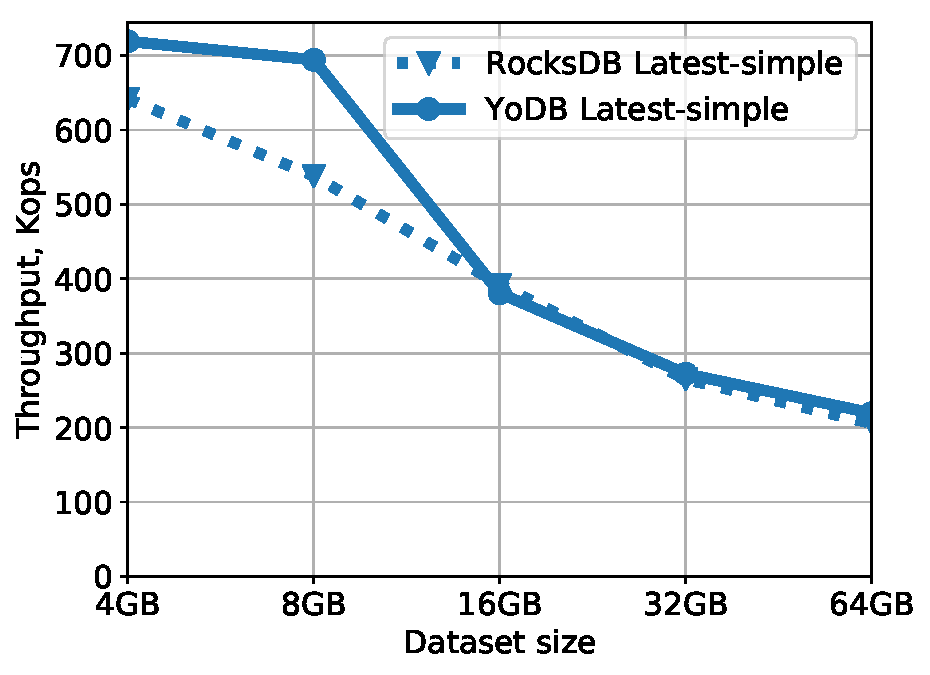
\includegraphics[width=0.3\textwidth]{figs/Workload_D_line.pdf}
\caption{{\sys\/ versus RocksDB throughput, under the YCSB-D workload and scaling dataset sizes.}}
\label{fig:throughput:d}
\end{figure}
}

\subsection{\sys\ Insights}
\label{ssec:drill} 

\paragraph{Vertical scalability.} 
Figure~\ref{fig:scalability} illustrates \sys's throughput scaling for the 64GB dataset under both Zipf  
distributions. We exercise the YCSB-A, YCSB-C and YCSB-P scenarios, with 1 to 12 worker threads.  
As expected, YCSB-C (read-only scenario) scales nearly perfectly (9.4x for composite keys, 7.7x for simple ones). 
The other workloads scale slower, due to read-write and write-write contention as well as background munk and funk rebalances. 
%YCSB-P scales 3.8x for both distributions at 8 threads. YCSB-A scales 6.4x for Zipf-composite and 4.6x for Zipf-simple at 12 threads. 
\inred{TODO update the graph and this paragraph when the new results are available. Ignore till then.}

\begin{figure}[th]
\centering
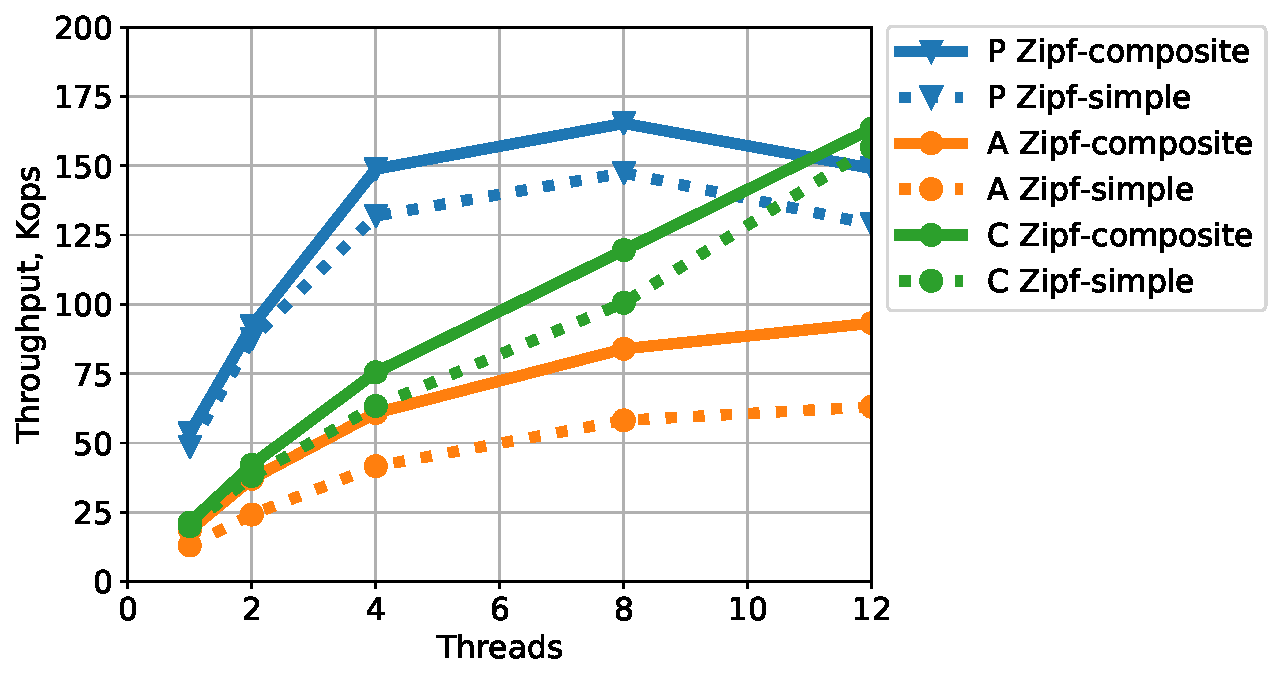
\includegraphics[width=0.35\textwidth]{figs/scalability_line.pdf}
\caption{{\sys\/ scalability with the number of threads for 
the 64GB dataset and different workloads. }}
\label{fig:scalability}
\end{figure}

\remove{
\begin{table*}
\centering
%\begin{subfigure}{0.55\linewidth}
{\small{
\begin{tabular}{l|cccccc|c|ccccc|}
\cline{2-7} \cline{9-13} 
  & \multicolumn{6}{c|}{Maximum log size} & & \multicolumn{5}{c|}{Bloom filter split factor}\\
%\cline{2-7} \cline{9-13} 
& 128KB & 256KB & 512KB & 1MB & 2MB & 4MB & &1 & 2 & 4 & 8 & 16 \\
\cline{2-7} \cline{9-13} 
Zipf-composite: & 50.2	& 55.5 & 80.7	& 134.1 & {\bf {157.5}} & 149.5 & & 134.7 & 133.5 & 140.1 & 152.5 & {\bf {157.4}}   \\
Zipf-simple:    & 27.8	& 30.9 & 36.1	& 58.3  & {\bf {68.3}}   & 68.1   & &  36.3 & 39.2   & 46.3  & 56.0  & {\bf {59.9}}\\
%\hline 
%YCSB-E, Zipf-range & 29.1	& 36.4 & 36.9	& 37.3	& {\inred{30.4}} & 	37.1 \\
%YCSB-E, Zipf & 16.1 & 16.3 &	15.8	& 15.8 &	16.4 &	15.8 \\
\cline{2-7} \cline{9-13} 
\end{tabular}
}}
%\caption{Throughput (Kops) vs log size}
%\label{fig:wal:sz}
%\end{subfigure}
%\hspace{0.09\linewidth}
%\begin{subfigure}{0.35\linewidth}
%{\small{
%\begin{tabular}{|l|c|c|c|c|}
%\hline 
%1 & 2 & 4 & 8 & 16\\
%\hline 
%134.7 & 133.5 & 140.1 & 152.5 & {\bf {157.4}} \\
% 36.3 & 39.2 & 46.3 & 56.0 & {\bf {59.9}} \\
%\hline 
%\end{tabular}
%}}
%\caption{Throughput (Kops) vs Bloom filter split factor}
%\label{fig:wal:bf}
%\end{subfigure}
\caption{{\sys\/ throughput under a mixed get-put workload (YCSB-A), 64GB dataset, and different configuration parameters.}}
\label{fig:wal}
\end{table*}
}

\begin{figure}[htb]
\centering
\begin{subfigure}{0.49\linewidth}
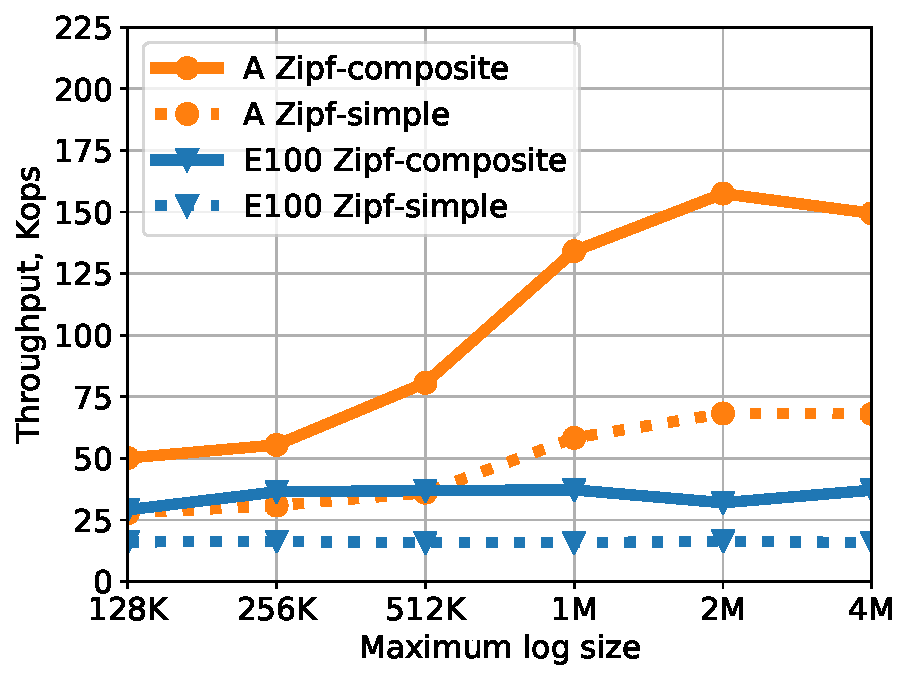
\includegraphics[width=\textwidth]{figs/max_log_size_line.pdf}
\caption{Maximum log size,\\  YCSB-A and YCSB-E100}
\label{fig:params:log}
\end{subfigure}
%\hspace{0.05\linewidth}
\begin{subfigure}{0.49\linewidth}
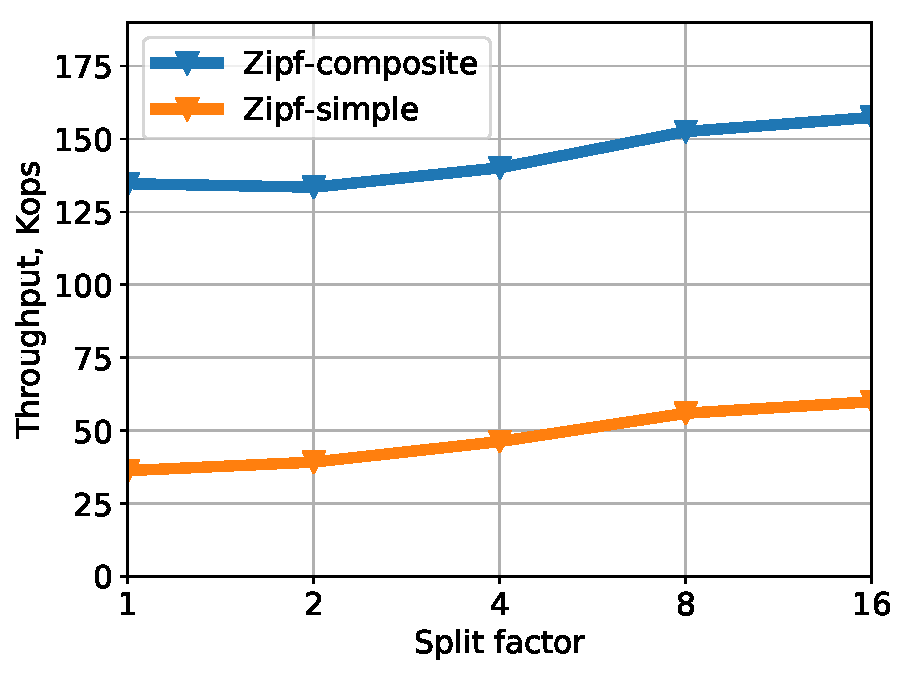
\includegraphics[width=\textwidth]{figs/Bloom_filter_line.pdf}
\caption{Bloom filter split factor,\\ YCSB-A}
\label{fig:params:bf}
\end{subfigure}
\caption{{\sys\/ throughput sensitivity to configuration parameters, on the 64GB dataset under the YCSB-A (mixed put-get) and 
YCSB-E100 (scan-dominant, 1 to 100 items).}}
\label{fig:params}
\end{figure}

\paragraph{Configuration parameters.} 
We explore the system's  sensitivity to funk-log configuration parameters, for the most challenging 64GB dataset, 
and explain the choice of the default values.

Figure~\ref{fig:params:log} depicts the throughput's dependency on the log size limit or munk-less funks, 
under the YCSB-A and YCSB-E100 workloads with Zipf-composite key distribution. 
The fraction of puts in YCSB-A is 50\% (versus 5\% in YCSB-E), which makes it more sensitive to the log size. 
A low threshold (e.g., 128KB) causes frequent funk rebalances, which degrades the performance more than 3-fold. 
On the other hand, too high a threshold (4MB) lets the logs grow bigger, and slows down gets. Our experiments are 
tuned to use 2MB logs, which favors write-intensive workloads. YCSB-E favors smaller logs, since the write 
rate is low, and more funk rebalances can be accommodated. Its throughput could grow by up to 20\% by tuning to
use 512KB logs.

Figure~\ref{fig:params:bf} depicts the throughput dependency on the Bloom filter split factor, under YCSB-A. 
Partitioning to 16 mini-filters gives the best result; beyond this point the benefit levels off. 
The impact of Bloom filter partitioning on the end-to-end get latency as well as the memory footprint is negligible.

\subsection{\sys\ versus PebblesDB}
\label{ssec:pebbles} 

We compared \sys\ and PebblesDB 
Table~\ref{fig:pebbels-throughput} presents the range of throughput lift of \sys\ over PebblesDB. 
%We compare both the Zipf-simple and Zipf-composite 
We compare workloads YCSB-P, and YCSB-A through YCSB-E. Experiments run Zipf-simple key distribution on 32GB data set, which is not our optimal execution point, and with 1 to 8 threads.
 \inred{TODO: time permitting, run pebblesDB with 12 threads, and also some mixed workload YCSB-A or YCSB-B or both}.
We note that across workloads the more threads being used the greater the lift is. We see similar trends also running with smaller data sets.
In general, RocksDB outperforms PebblesDB. This can be attributed to running on different hardware, using container and running with more threads than in the experiments presented in~\cite{PebblesDB}.


\begin{table}
\centering
{\small{
\begin{tabular}{|l|c|}
%Workload & Zipf-simple & Zipf-composite \\
\hline 
Workload & lift range \\
\hline 
YCSB-P & 1.5-2.9x \\
%YCSB-A & x.x-x.x  \\
%YCSB-B & x.x-x.x \\
YCSB-C & 2.1-3.2x\\
YCSB-E10 & 2.2-4.5x \\
YCSB-E100 & 2.2-3.8x \\
YCSB-E1000 & 2.4-4.2x \\
\hline 
\end{tabular}
}}
\caption{{\sys\/ lift over PebblesDB, running on 32GB with 1 to 8 threads}}
\label{fig:pebbels-throughput}
\end{table}




  